\chapter{Együttműködések}
%(6 oldal): Hogyan csatlakoztak be, mit értek el, mivel lett több az egész, együttműködések menete.

A mérési rendszer fejlesztése 2015 tavaszi félévében kezdődött önálló laboratóriumi munkaként. Az első működő verziót követően további témakiírások készültek hozzá kapcsolódóan. Ezek közreműködési lehetőséget biztosítottak a hallgatóknak, hogy saját munkájuk során a meglévő mérési rendszert vagy annak eredményeit felhasználják és kiegészítsék azt. A következőkben ezen munkák kerülnek bemutatásra. Az egyes leírások fontos eleme a mérési rendszerhez való hozzáadott értékek és a rendszer felhasznált szolgáltatásainak kiemelése.

Ezen együttműködéseknél rendkívül fontos volt az ismeret átadás, és a munkák koordinálása. A konzulensemmel, Dr Heszberger Zalánnal, végig gondot fordítottunk arra hogy minden szükséges tudást átadjunk a munkákhoz, és felügyeljük azok végrehajtását. Minden esetben elégedettek voltunk a közös munka gyümölcsével, és sokszor kellemesen meglepett milyen távolra vezettek az általunk elindított témák.

Az egyes fejezetcímek az elkészült dolgozatok címének felelnek meg.

\section{Forgalmi mérési környezet kialakítása az Interneten}
%Haja Dávid munkájának rövid bemutatása (2 oldal)

% Mit adott hozzá az én témámhoz?
% Az én témámnak mely részeire tudta építeni a saját munkáját?

Haja Dávid alapszakos hallgató a szakdolgozataként választotta az általunk kiírt témát 2015 őszi félévében. Munkája során megismerte az Elméleti Áttekintés fejezet tudásanyagát, valamint a mérőrendszer felépítését. Fő tevékenységei a PlanetLab hálózat komolyabb megismerése volt, valamint a mérési rendszer kiegészítése sávszélesség kapacitás méréssel.

\subsection*{PlanetLab rendszerének megismerése}
A mérések végrehajtása során a PlanetLab hálózat gépeinek elérésével gondjaink akadtak. A tanszéken üzemelő szerverek nem megfelelően voltak felkonfigurálva, nem üzemeltek rendeltetésszerűen. A kölcsönösség elve alapján így nem fértünk hozzá a PlanetLab hálózatának szervereihez.
Haja Dávid közreműködésével az említett szerverek helyre lettek állítva. Ezen munkája során mély ismeretekre tett szert a PalnetLab szervezet működésével és a szerverek felépítésével kapcsolatban.

\subsection*{D-ITG sávszélesség mérés}
A mérési rendszer eredetileg csak iperf sávszélesség mérésekkel rendelkezett, mivel ez a szoftver a legtöbb linux alapú rendszereken, így a PlanetLab gépein is, előre telepítve volt. A mérések színvonalának érdekében azonban Haja Dávid feladata volt felmérni mely további sávszélességmérő rendszerek nyújthatnak megbízható és részletes mérési adatokat. Kutatásai során választása a D-ITG-re (Distributed Internet Traffic Generator) esett. Ez a mérőszoftver bír az elvárható alapképességekkel, mint a kinyerhető adatok széles választéka, protokoll támogatások, párhuzamos folyamok kezelése, valamint sztochasztikus adatküldő profilok is beállíthatóak. A program azonban nem elérhető a publikus csomagkezelő rendszerekből, ahonnan egyszerűen telepíthetőek lennének. Emiatt munkájának nagy része volt a szoftver becsomagolása a PlantLab gépeinek megfelelő RPM formátumba. 
Az így elkészült telepítőcsomagok automatizált telepítését az Ansible szoftverrel oldotta meg.

Munkájának gyümölcseként új mérési lehetőségekkel bővült az eredeti rendszer. Az új mérési típus nem jöhettek volna létre a mérési rendszer rugalmassága által, a rendszer forráskódjában egyetlen osztály létrehozására volt szükség az új funkció implementálásához. Az új képességeket jól mutatja be az alábbi mérési eredmény, amely két különböző, ám hálózati szempontból közel lévő cél felé indít sávszélesség méréseket. Mind a négy részeredmény ugyanahhoz a mérési forgatókönyvhöz tartozik. Alább részletezem az egyes részmérések tartalmát:

\begin{itemize}
\item 10 másodperces mérés az első cél felé
\item 10 másodperces mérés a második cél felé
\item 10 másodperces mérés parallel a két cél felé, az első cél folyamának eredményeit prezentálva
\item 10 másodperces mérés parallel a két cél felé, a második cél folyamának eredményeit prezentálva
\end{itemize}

\begin{center}
%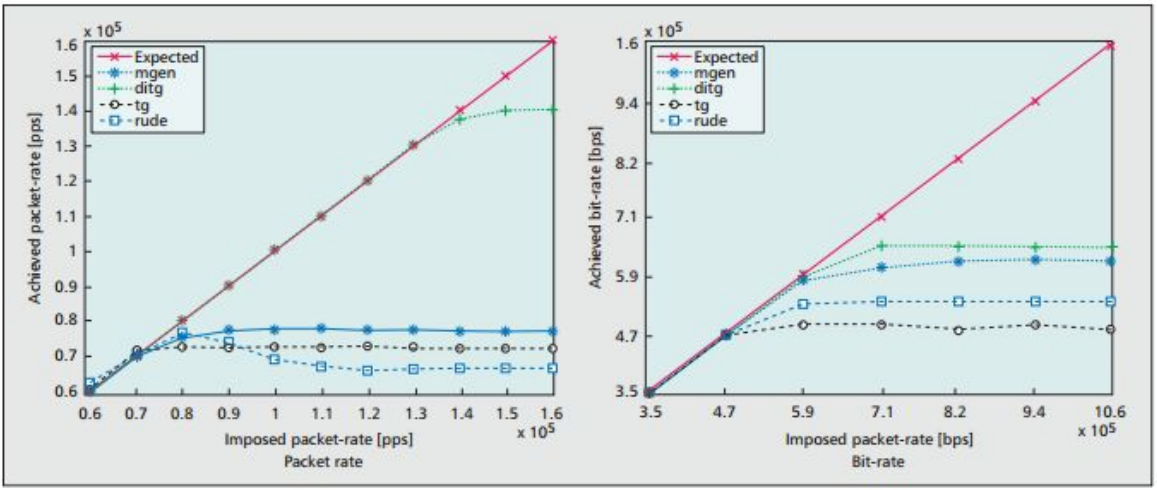
\includegraphics[width=0.8\textwidth,keepaspectratio]{figures/d-itg-diagram.PNG}
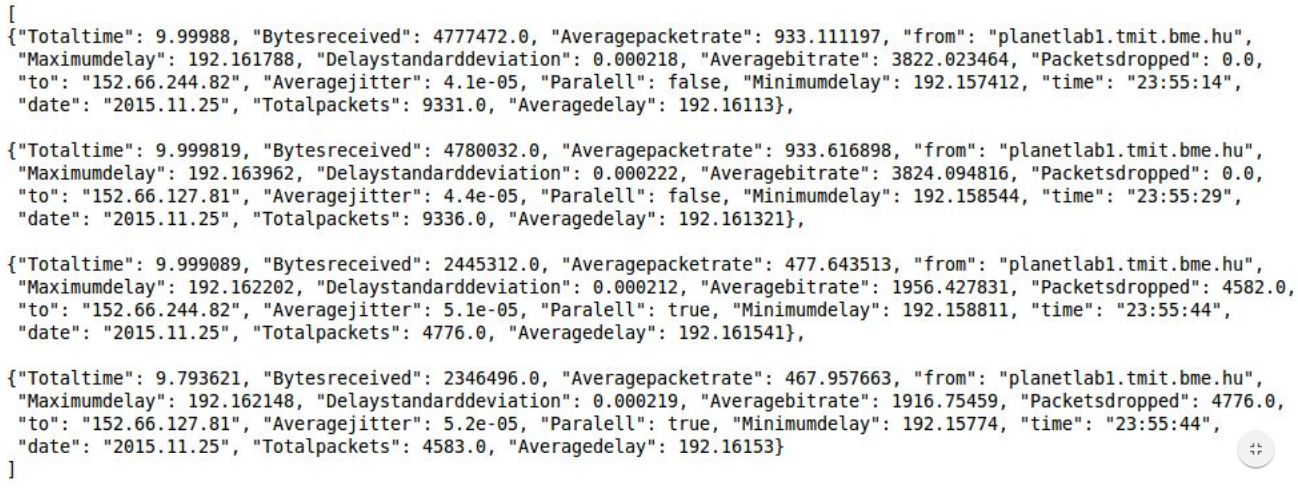
\includegraphics[width=0.8\textwidth,keepaspectratio]{figures/d-itg-measure.PNG}
\end{center}


\section{AS útvonalváltozások vizsgálata}
Kocsmár Bence munkájának rövid bemutatása (2 oldal)

\section{Adatbázis szervezés webes környezetben}
%Patkó Ákos munkájának rövid bemutatása (1-2 oldal)

Patkó Ákos alapszakos hallgató önálló laboratóriumi témaként választotta a mérési rendszerhez tartozó kiírásunkat 2016 tavaszi félévében. Munkája során a korábbi üzemeltetési problémák megoldásán dolgozott, valamint egyéb fejlesztéseket eszközölt a könnyebb telepíthetőség és üzemeltethetőség érdekében.















